\chapter[Resultados e Discussão]{Resultados e Discussão}

\section{Teste do Algoritmo}

O algoritmo foi aplicado a cada um dos bancos de dados indicados na sessão anterior, de maneira a determinar os subconjunto ótimos de variáveis para uso em um modelo de regressão. O resultado obtido determina, a cada iteração, a variável ainda não utilizada que, ao ser acrescentada no modelo, traz a maior redução do erro de validação cruzada (ou o menor aumento). 

A cada iteração "\textit{i}", um subconjunto candidato de \textit{i} variáveis é determinado. O melhor subconjunto é aquele que minimiza o erro LOOCV. É importante reiterar que o algoritmo utiliza uma estratégia de \textit{greedy search} para buscar os subconjuntos e, portanto, a optimalidade global desses subconjuntos não é garantida.

\subsection{Resultados}

\subsubsection{\textit{Communities and Crime}}

No banco de dados \textit{Forest Fires}, o erro de validação cruzada LOOCV mínimo foi observado em um conjunto com apenas 37 das 102 variáveis. A adição de variáveis posteriormente teve pouca influência no erro de validação cruzada, com uma tendência de overfitting na inclusão das últimas variáveis.

O resultado para cada iteração pode ser verificado na figura \ref{fig:stepwise_CommunitiesandCrime_validation}.

\begin{figure}[!htb]
    \centering
    \caption{Seleção de Variáveis \textit{Stepwise: Communities and Crime}.}
    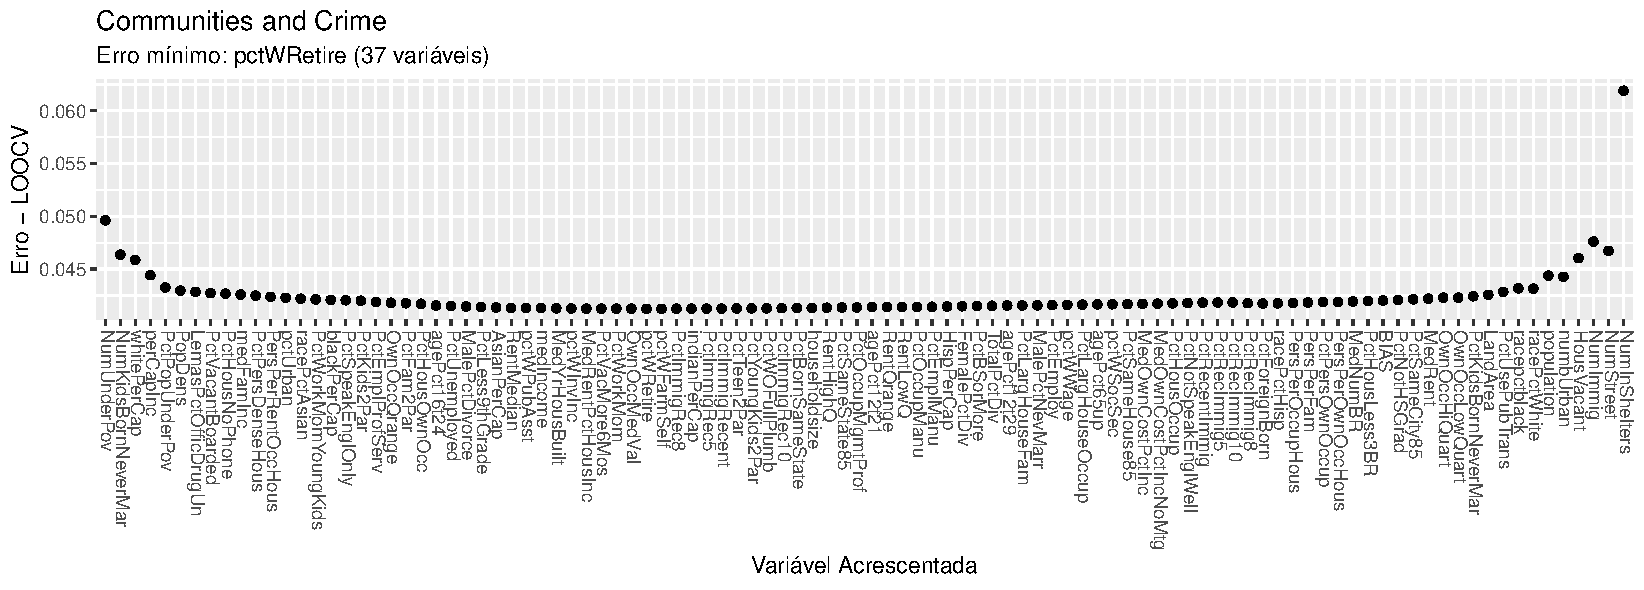
\includegraphics[height=163pt]{imgs/res/CommunitiesandCrime_validation.pdf}
    \legend{Fonte: Própria.}
    \label{fig:stepwise_CommunitiesandCrime_validation}
\end{figure}

\subsubsection{\textit{Forest Fires}}

No banco de dados \textit{Forest Fires}, o erro de validação cruzada LOOCV mínimo foi observado em um conjunto com apenas 4 das 12 variáveis. A adição de variáveis posteriormente resultou em overfitting significativo. 

O resultado para cada iteração pode ser verificado na figura \ref{fig:stepwise_ForestFiresDataset_validation}.

\begin{figure}[!htb]
    \centering
    \caption{Seleção de Variáveis \textit{Stepwise: Forest Fires}.}
    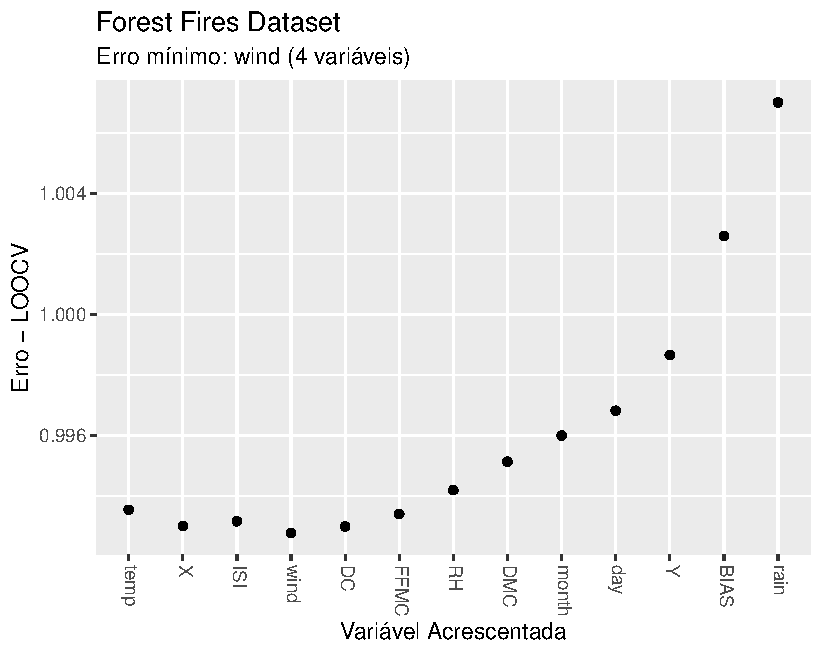
\includegraphics[height=200pt]{imgs/res/ForestFiresDataset_validation.pdf}
    \legend{Fonte: Própria.}
    \label{fig:stepwise_ForestFiresDataset_validation}
\end{figure}

\subsubsection{\textit{USA Housing}}

No banco de dados \textit{USA Housing}, o erro de validação cruzada LOOCV mínimo foi observado em um conjunto com apenas 35 das 80 variáveis. A adição de variáveis posteriormente teve pouca influência no erro de validação cruzada, porém aumentando-o lentamente. 

O resultado para cada iteração pode ser verificado na figura \ref{fig:stepwise_USAHousingDataset_validation}.

\begin{figure}[!htb]
    \centering
    \caption{Seleção de Variáveis \textit{Stepwise: USA Housing}.}
    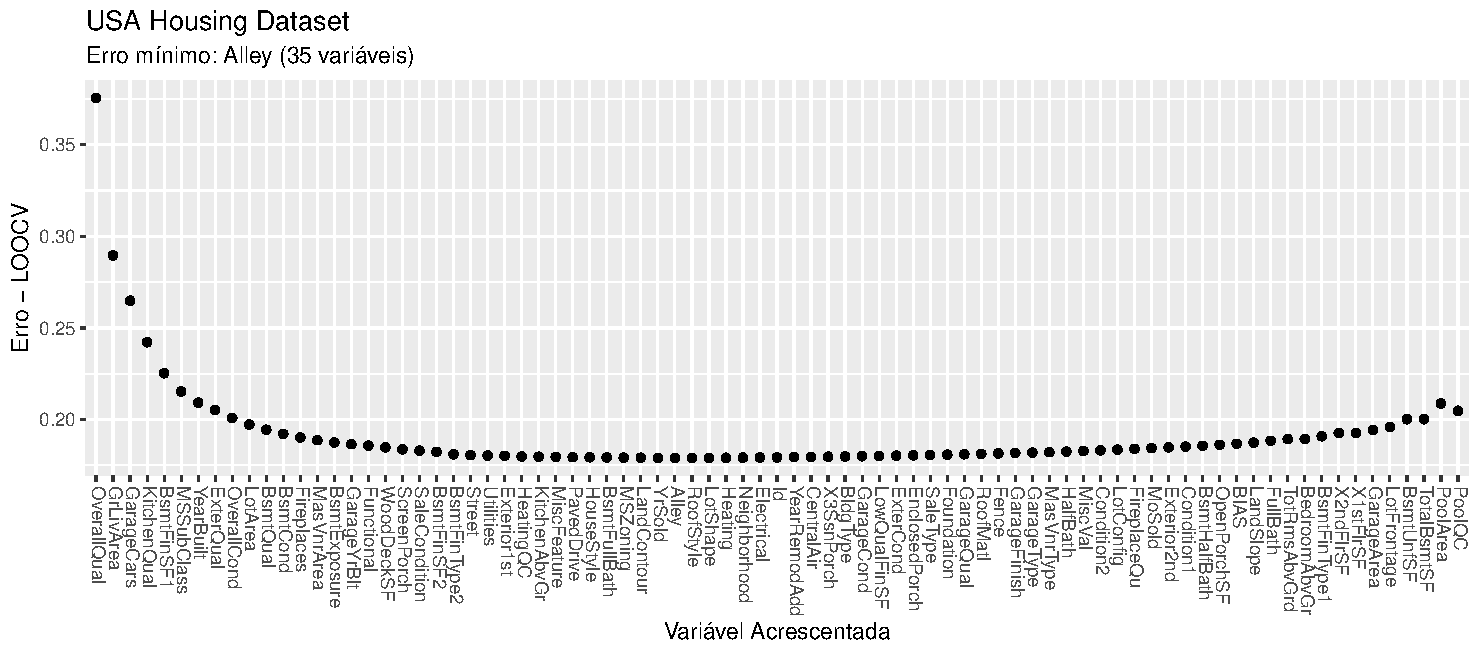
\includegraphics[height=200pt]{imgs/res/USAHousingDataset_validation.pdf}
    \legend{Fonte: Própria.}
    \label{fig:stepwise_USAHousingDataset_validation}
\end{figure}

\subsubsection{\textit{Wisconsin Breast Cancer}}

No banco de dados \textit{Wisconsin Breast Cancer}, o erro de validação cruzada LOOCV mínimo foi observado em um conjunto com apenas 8 das 32 variáveis, e foi identificada também uma tendência significativa ao overfitting quando utilizado um subconjunto candidato de mais de 16 variáveis. 

O resultado para cada iteração pode ser verificado na figura \ref{fig:stepwise_WisconsinBreastCancer}.

\begin{figure}[!htb]
    \centering
    \caption{Seleção de Variáveis \textit{Stepwise: Wisconsin Breast Cancer Dataset}.}
    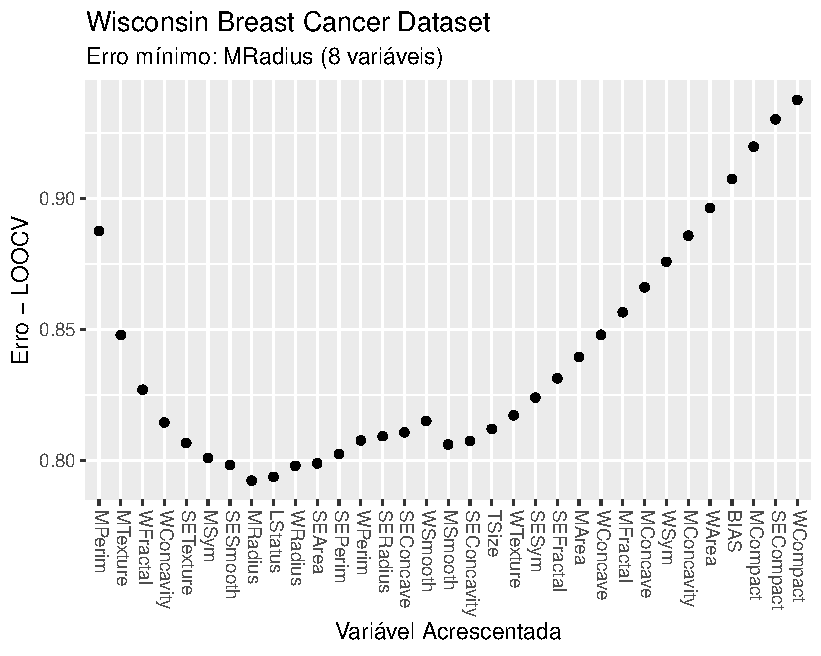
\includegraphics[height=200pt]{imgs/res/WisconsinBreastCancerDataset_validation}
    \legend{Fonte: Própria.}
    \label{fig:stepwise_WisconsinBreastCancer}
\end{figure}


\subsection{Discussão}

Observou-se o decréscimo do erro com o aumento do número de variáveis selecionadas até um ponto de mínimo, a partir do qual a tendência se inverte e o erro passa a aumentar. Tal dinâmica é esperada, uma vez que o aumento do número de parâmetros, na regressão linear, resulta no aumento da complexidade do modelo \cite[p. 224]{statistical_learning}. 

De fato, ao se reduzir a complexidade do modelo através do aumento do parâmetro de regularização ($\lambda$), observa-se a diminuição da tendência ao overfitting, conforme demonstra a figura \ref{fig:lambda_WisconsinBreastCancer}.

\begin{figure}[!htb]
    \centering
    \caption{Efeito do parâmetro de regularização ($\lambda$): \textit{Wisconsin Breast Cancer Dataset}.}
    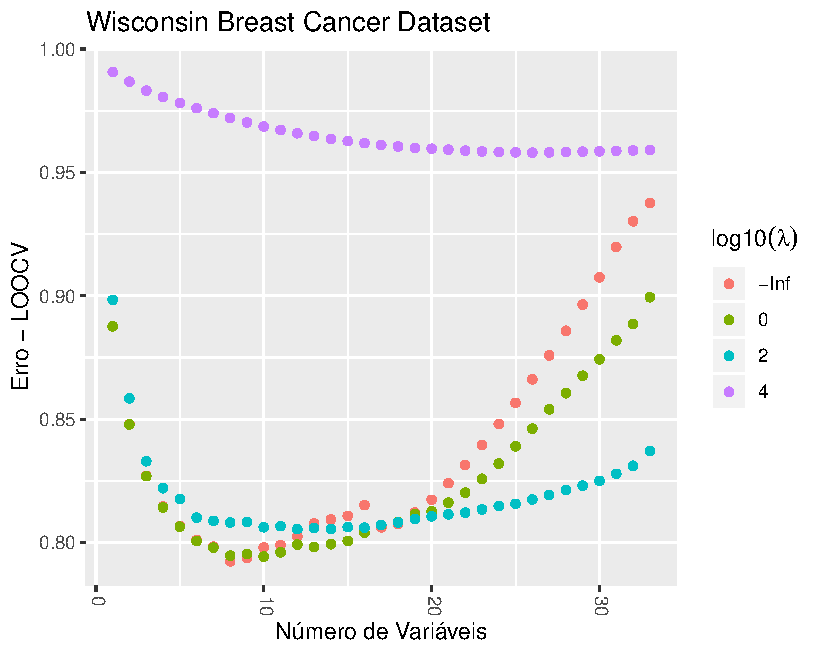
\includegraphics[height=200pt]{imgs/res/WisconsinBreastCancerDataset_lambda}
    \legend{Fonte: Própria.}
    \label{fig:lambda_WisconsinBreastCancer}
\end{figure}

É interessante notar que valores de $\lambda$ reduzidos tiveram pouca ou nenhuma influência nos primeiros subconjuntos ótimos selecionados pelo algoritmo, alterando apenas a seleção na região com tendência ao overfitting. Dessarte, a utilização de um parâmetro de regularização não nulo de pequena magnitude tem pouca influência no conjunto selecionado, enquanto melhora a estabilidade numérica do método, evitando operações com matrizes singulares.

\section{Estudo de Caso: Vallourec - Caracterização de tubos de aço}